\documentclass[tikz, border=10pt]{standalone}
\tikzset{
    vertex/.style = {
        circle,
        fill            = black,
        outer sep = 15pt,
        inner sep = 15pt,
    }
}
\begin{document}
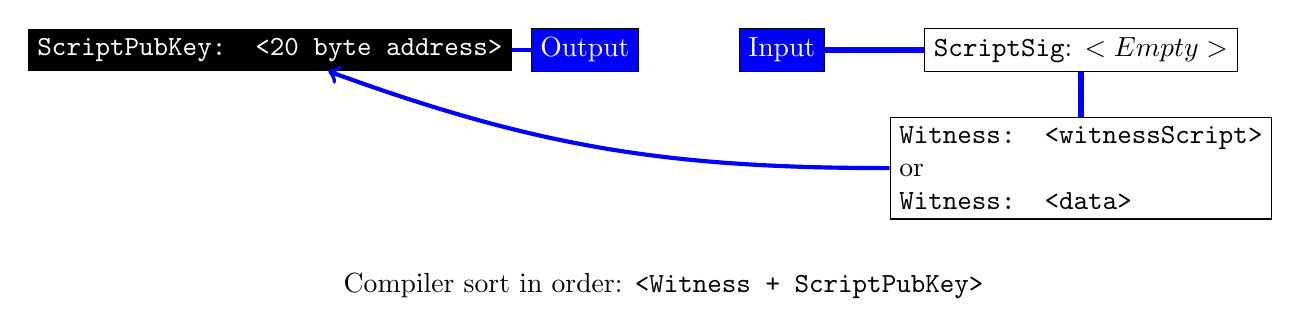
\begin{tikzpicture}
  % Coinbase

  \node[draw,fill=black,text=white] (scpk0) at (0,0) {\texttt{ScriptPubKey: <20 byte address>}};

  \node[draw,fill=blue,text=white] (out0) at (4,0) {Output};

  \draw[-,draw=blue,line width=1.5pt] (scpk0) to (out0);
  

  \node[draw,fill=blue,text=white] (in0) at (6.5,0) {Input};



  \node[draw] (scsg1) at (10.3,0) {\texttt{ScriptSig}: $<Empty>$};

  \node[draw,align=left] (scsg2) at (10.3,-1.5) {\texttt{Witness: <witnessScript>}\\or\\\texttt{Witness: <data>}};

  \draw[<-,draw=blue,line width=1.5pt] (scpk0) to[in= 180,out=-20] (scsg2);

  \draw[-,draw=blue,line width=2pt] (in0) to (scsg1);
  \draw[-,draw=blue,line width=2pt] (scsg1) to (scsg2);
 
%   \node () at (8.8,0) {...};
  
  \node at (5, -3) {Compiler sort in order: \texttt{<Witness + ScriptPubKey>}};

  
    

\end{tikzpicture}
\end{document}